\section{Conception Devops}
\begin{figure}[h]
   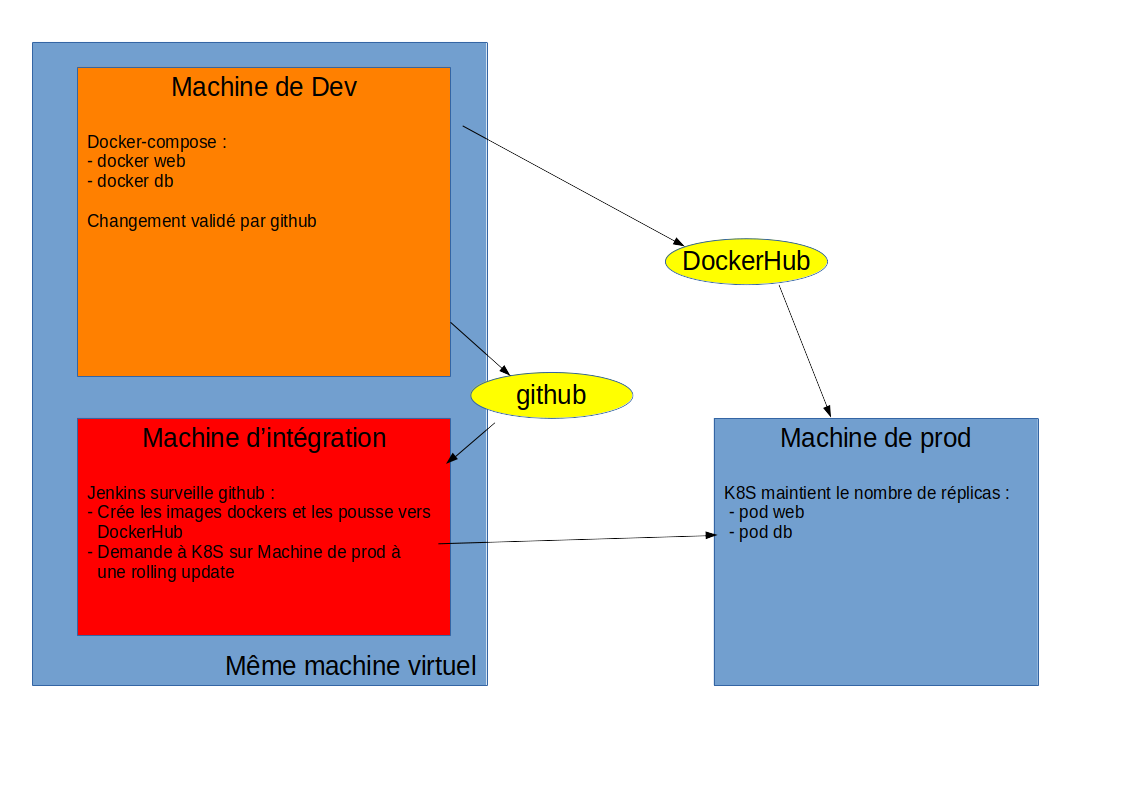
\includegraphics[width=1.0\textwidth]{schema.png}
\end{figure}
\subsection{Gestion de versions}
Tous les ficheirs sources et de configuration sont versionné avec git en utilisant github :

\url{https://github.com/RaoulChartreuse/exo_SNCF}


On utilisera 2 branches principale, une branche dev pour l'implementation des nouvelles fonctionalités et une branche release pour chaque version validée.

\subsection{Machine de production}
Compte tenue des besoins de disponibilité et de mise à l'echelle (scalling), la conteneurisation retenue est \emph{kubernetes} qui permet justement de géner le nombre de réplication et de garentir celui-ci.

Compte tenue de l'environement du projet, nous utiliseront \emph{minikube} et simulerons un ensemble de serveur sur une machine virtuelle de dévellopement.

Liste des pods~:
\begin{itemize}
\item web : un pod de serveurs appache/php
\item db : un pod de serveurs mysql
\end{itemize}

\subsection{Machine de Dévellopement}
Idéalement l'environement de test doit identique à m'environement de production. Ici en l'abscence de machine de test et avec des resources limité à un seul ordinateur, nous utiliseront pour le dévellopement des serveurs dockers obtenue grace à un \emph{docker compose}.

Liste des serveurs~:
\begin{itemize}
\item web : un docker appache/php
\item db : un docker mysql
\end{itemize}

\subsection{Deploymenent et integration}
La surveillance des dépots git sera éffectué par un serveur emph{Jenkins}. Dans le cadre des ressources limitées du projet jenkin sera contenérisé par un conteneur docker sur la machine de dévellopement.

\subsubsection{Mise à jour de la branche dev}
En cas de mise à jour de la branche dev il faut~:
\begin{itemize}
\item Arreter les conteneurs db
\item Recréer les images des conteneurs à jour grace à docker compose
\item Lancer ses conteneurs à jour
\item Supprimer les images obsoléte
\end{itemize}

\subsection{Mise à jour de la branche prod}
Nous utiliserons la fonctionalité Rolling update de kubernetes.

\subsection{Création des machines de prod}
Nous automatiserons la création des machines de prod grace à \emph{Ansible}.
Ici dans le cadre du projet cela ce limitera à la configuration d'une seul machine de prod, l'instalation et le déployment de minikube.

%%% Local Variables:
%%% mode: latex
%%% TeX-master: t
%%% End:

